\chapter{Escopo do Projeto }

O escopo de um projeto é essencial para que seja realizado o planejamento do mesmo. A partir dele, delimita-se o que deve ser realizado, em quanto tempo será realizado, quanto custará, quem irá realizá-lo, quais os produtos e/ou serviços deverão sem entregues e a descrição sumária do projeto.

Para melhor visualização do mesmo, foram usadas algumas diferentes ferramentas:

\textbf{5W2H - Projeto}
What – O que será entregue?

Projeto de um Sistema de Comunicação Interveicular para Alertas de Colisões em Rodovias Brasileiras (CIAC).

Why – Por que está sendo feito?

Devido à alta quantidade de acidentes em rodovias de mão dupla brasileiras oriundos de colisões frontais, que representam apenas 4\% dos casos, porém 24,6\% do total de fatalidades. O alto custo despendido pelo Governo Brasileiro com os acidentes em geral, justificaria o investimento necessário para o planejamento, execução e implantação do projeto CIAC.

Where – Onde será feito/entregue/utilizado?


Na Universidade de Brasília, Campus Faculdade Gama, onde serão realizados dois encontros semanais nas segundas-feiras e quartas-feiras, respectivamente, das 16h00 às 17h50, além de encontros extras esporádicos quando necessário.

When – Quando será feito/entrega?

O Projeto CIAC terá duração de um semestre letivo, a partir de agosto até dezembro de 2015.

Who – Quem o fará?

O Projeto será realizado pelo Grupo 5 da disciplina Projeto Integrador 1 do Campus Faculdade Gama – UnB, onde o grupo é composto por estudantes de 5 engenharias: Automotiva, Aeroespacial, de Energia, Eletrônica e de Software.


How – Como será realizado?

Por meios adquirido pelos integrantes do grupo serão divididos de acordo com as suas áreas de atuação, envolvendo as engenharias para um melhor e maior alcance da abordagem do problema. A metodologia utilizada para a realização do projeto será o Scrum.

How Much – Quanto custará?

Além do tempo dos participantes desse projeto, é previsto apenas o custo relativo à impressão dos relatórios.


\textbf{5W2H - Produto}
What – O que será entregue?

Será entregue o projeto de um Sistema de Comunicação Interveicular para Alertas de Colisões em Rodovias Brasileiras (CIAC).

Why – Por que está sendo feito?

Devido à alta quantidade de acidentes em rodovias de mão dupla brasileiras oriundos de colisões frontais, que representam apenas 4\% dos casos, porém 24,6\% do total de fatalidades. O alto custo despendido pelo Governo Brasileiro com os acidentes em geral, justificaria o investimento necessário para o planejamento, execução e implantação do projeto CIAC.

Where – Onde será utilizado?

O CIAC será instalado em veículos automotores terrestres, com a exceção de ciclomotores e motocicletas.

When – Quando será feito/entrega?

A estimativa irá depender do prazo necessário para que os dispositivos integrantes do CIAC para produção e deslocamento dos mesmos até o local onde será feito a montagem do Sistema. O que podemos afirmar é que o planejamento do projeto será feito dentro do prazo de 4 meses.

Who – Quem o fará?

O projeto será desenvolvido por estudantes dos cursos de engenharia especializados nas áreas de Automotiva, Aeroespacial, Eletrônica, de Energia e de Software para implantação do mesmo.

How – Como será realizado?

Será constituído por diferentes dispositivos, sendo os principais o Transponder, o GPS, o Radar, o Lidar, a Câmera e um sensor de rotação angular, além do Microprocessador que fará a integração dos mesmos, responsáveis pela transmissão, interpretação e recepção dos dados relativos aos veículos automotores terrestres envolvidos na situação de aplicação do sistema.

How much – Quanto custará?

Será feito um estudo de custos e viabilidade do mesmo ao longo das próximas etapas.

\textbf{Diagrama de Fishbone}

Também conhecido como Diagrama de Causa e Efeito, é um método para análise de causas-raiz e tem como objetivo otimizar a identificação das causas que geram determinados problemas que precisam ser solucionados ou fatores que levam a resultados que se deseja obter, através da representação gráfica.

\begin{figure}[h!]
\centering
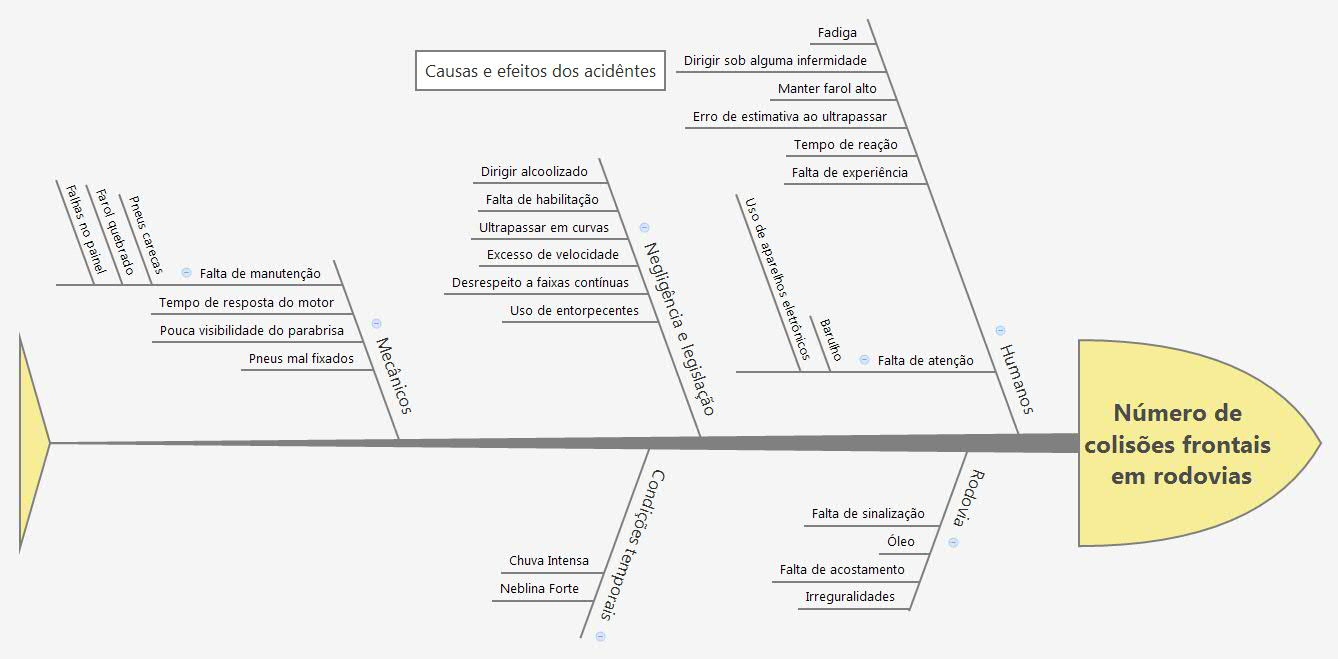
\includegraphics[width=250px, scale=1]{figuras/fishbone}
\caption{Diagrama de Fishbone do Projeto}
\label{fig:fishbone}
\end{figure}


\textbf{EAP do Projeto}
\begin{figure}[h!]
\centering
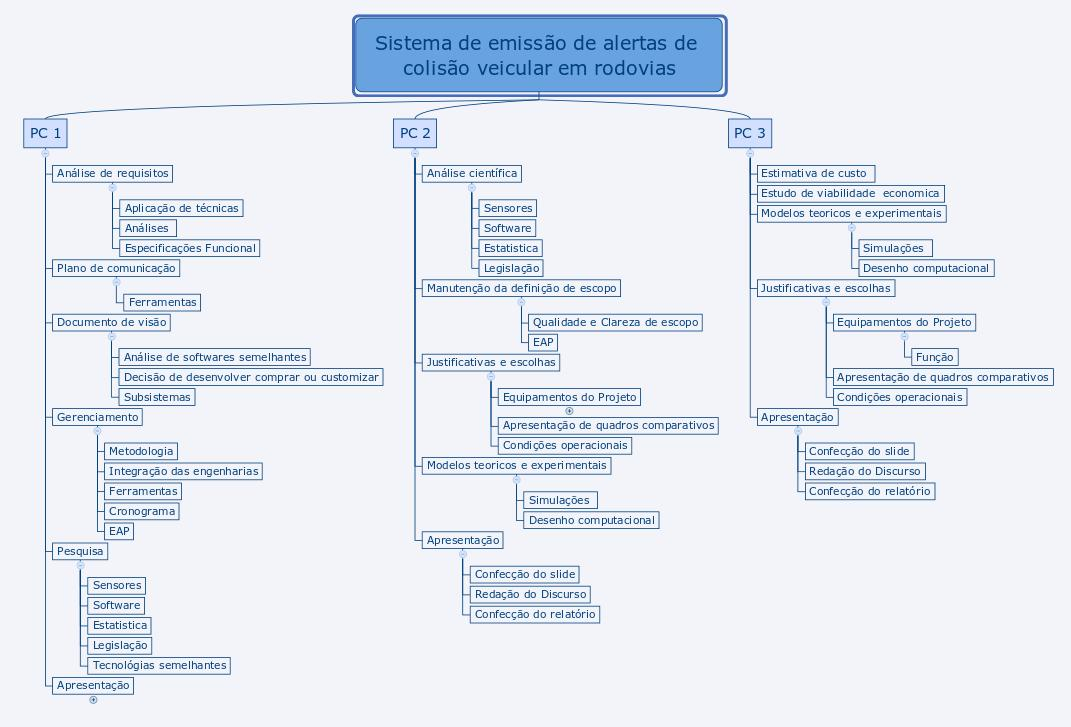
\includegraphics[width=250px, scale=1]{figuras/neweap}
\caption{EAP do Projeto}
\label{fig:neweap}
\end{figure}

\textbf{Sistema de emissão de alertas de colisão veicular em rodovias}
\\

\begin{table}[]
\centering
\caption{Ponto de Controle 1 – PC 1}
\label{custo_equip}
\begin{tabular}{|p{4cm}|p{5cm}|}
  \hline
  Análise de Requisitos & Aplicação de técnicas, Análises, Especificações funcionais do sistema. \\
  \hline
  Plano de Comunicação & Ferramentas. \\
  \hline
  Documento de Visão & Análise de softwares semelhantes, Decisão de desenvolver ou customizar, Subsistemas. \\
  \hline
  Gerenciamento & Metodologia, Integração das engenharias, Ferramentas, Cronograma, EAP. \\
  \hline
  Pesquisa & Sensores, Software, Estatística, Legislação, Tecnologias semelhantes. \\
  \hline
  Apresentação & Confecção do slide, Redação do discurso, Confecção do relatório. \\
  \hline

\end{tabular}
\end{table}



\begin{table}[]
\centering
\caption{Ponto de Controle 2 – PC 2}
\label{custo_equip}
\begin{tabular}{|p{4cm}|p{5cm}|}
  \hline
  Análise Científica & Sensores, Software, Estatística, Legislação. \\
  \hline
  Manutenção da Definição de Escopo & Qualidade e clareza do escopo, EAP. \\
  \hline
  Justificativas e Escolhas & Equipamentos do Projeto, Apresentação de quadros comparativos, Condições operacionais. \\
  \hline
  Modelos teóricos e experimentais & Simulações, Desenho computacional. \\
  \hline
  Apresentação & Confecção do slide, Redação do discurso, Confecção do relatório. \\
  \hline

\end{tabular}
\end{table}


\begin{table}[]
\centering
\caption{Ponto de Controle 3 – PC  3}
\label{custo_equip}
\begin{tabular}{|p{4cm}|p{5cm}|}
  \hline
  Estimativa de Custo & Pesquisa de sistemas já existentes, Custo dos dispositivos escolhidos. \\
  \hline
  Estudo de Viabilidade Econômica & Custos dos dispositivos escolhidos, Justificativa. \\
  \hline
  Modelos Teóricos e Experimentais & Simulações, Desenho computacional. \\
  \hline
  Justificativas e Escolhas & Equipamentos do projeto, Apresentação de quadros comparativos, Condições operacionais. \\
  \hline
  Apresentação & Confecção do slide, Redação do discurso, Confecção do relatório. \\
  \hline
\end{tabular}
\end{table}


Nome do Projeto

Sistema de Comunicação Interveicular para Alertas de Colisões em Rodovias Brasileiras (CIAC).

Objetivos do Processo

Tem por objetivo a declaração de escopo do projeto do CIAC, evidenciando as necessidades e restrições a serem solucionadas durante a evolução do projeto.

Justificativa do Projeto

Auxiliar os condutores a realizar ultrapassagens com total segurança e eficácia, evitando assim possíveis acidentes causados principalmente por colisões frontais em rodovias de mão dupla no território brasileiro.

Descrição do Projeto

O CIAC apresenta uma solução para a alta incidência de acidentes fatais em rodovias brasileiras de mão dupla, oriundos de ultrapassagens malsucedidas. Por meio de uma comunicação interveicular que ocorre em tempo real entre dispositivos capazes de fornecerem os dados necessários para que o sistema calcule o tempo de ultrapassagem e a distância entre os veículos, será informado ao condutor se a ultrapassagem poderá ser realizada com segurança ou não. Para total eficiência do sistema, o mesmo deve ser instalado em todos os veículos automotores terrestres, com exceção de ciclomotores e motocicletas.

Produto do Projeto
O produto será um Sistema de Comunicação Interveicular para Alertas de Colisões em Rodovias Brasileiras (CIAC) que tem como objetivo auxiliar o condutor a realizar ultrapassagens em rodovias de mão dupla com total segurança, a fim de evitar um dos tipos de acidentes que mais gera vítimas fatais nesse meio, a colisão frontal. Esse sistema será composto principalmente por dispositivos como o Transponder, o GPS, o Radar, o Lidar, a Câmera e um sensor de rotação angular, além do Microprocessador que fará a integração dos mesmos, responsáveis pela transmissão, interpretação e recepção dos dados relativos aos veículos automotores terrestres, exceto ciclomotores e motocicletas, envolvidos na situação de risco.




Critérios de aceitação do produto do projeto:

Para tal, devem-se cumprir os requisitos estabelecidos tanto para o planejamento do sistema quanto para a sua execução. Para que isso ocorra deve-se levar em consideração, que todos os veículos automotores terrestres, exceto ciclomotores e motocicletas, possuam o sistema em pleno funcionamento, os requisitos que ativam o sistema, o Código de Trânsito Brasileiro (CTB) e ainda a diminuição de acidentes do tipo colisão frontal em rodovias de mão dupla.

Exclusões específicas e limites do projeto:

O produto do projeto apresenta uma série de restrições que foram especificadas ao longo do projeto, tais como os tipos de rodovias (simples de mão dupla e dentro do território brasileiro) em que o sistema funcionará, os tipos de veículos participantes (todos veículos automotores terrestres, com exceção de ciclomotores e motocicletas), condições climáticas de acordo com cada dispositivo (fortes tempestades e neblinas afetam o funcionamento de alguns dispositivos, como o LIDAR), a não identificação de outros objetos que não sejam veículos automotores terrestres, exceto ciclomotores e motocicletas, o sistema não será acionado dentro de perímetros urbanos (cidades) e ainda alertará ao condutor que a ultrapassagem não é segura quando o carro estiver em curvas ou subidas, pois de acordo com o Código de Trânsito, realizar essa manobra nessas situações é contra a lei.

Com relação ao consumo energético do projeto, a bateria já existente no veículo será suficiente para a alimentação de todo o sistema. Além das restrições supracitadas poderão surgir novas complicações ocasionadas por falha de algum dos dispositivos, eventuais acidentes causados por falhas humanas e caso o alternador da bateria do automóvel para de funcionar.

Características e requisitos do produto do projeto:

As características fazem parte do domínio da solução do projeto, incluindo seus requisitos funcionais e não funcionais. Os requisitos funcionais se referem as funcionalidades do projeto enquanto os requisitos não funcionais se referem aos termos de desempenho, usabilidade, confiabilidade, segurança, disponibilidade, manutenção e tecnologias envolvidas.

Dessa forma, os requisitos funcionais são:

\begin{itemize}
  \item O sistema deve emitir um alerta sonoro para o condutor ficar em alerta, caso não seja possível a ultrapassagem.
  \item O sistema deve calcular a distância entre os veículos em tempo real, para que seja possível a emissão dos dados aos outros dispositivos de segurança.
  \item O sistema deve emitir um alerta visual na tela do dispositivo do carro para o condutor observar o que está acontecendo na rodovia
  \item O sistema deve emitir sinais de rádio para informar aos aparelhos dos outros carros que contém o sistema de sua presença na rodovia.
  \item O sistema deve informar na tela do dispositivo a direção dos carros na rodovia para o usuário.
  \item O sistema deve mostrar na tela do dispositivo para o usuário os tipos de veículos que estão no raio de funcionamento do sistema.
  \item O sistema deve ser capaz de fazer processamento de imagem para mostra-los na tela do dispositivo.
  \item O sistema deve capturar a localização do veículo para informar os dados para os outros veículos que estão no raio de funcionamento do sistema.
  \item O sistema deve conter uma câmera para fazer a análise das posições dos carros na rodovia.
  \item O sistema deve conter um aparelho de detecção via laser para medir distâncias entre os veiculos que estão em direções opostas.
  \item O sistema deve conter um radar para detecção de objetos na rodovia.
  \item O sistema deve conter um sensor de rotação para aferir a posição angular do volante do veículo.

  \item Os requisitos não funcionais são:

\item   Tempo de resposta <= 10 ms;
  \item Deve funcionar em ambientes com fortes trepidações;
  \item Deve funcionar sobre condições climáticas adversas (Chuvas, Neve, Neblina, etc);
  \item O sistema deve sempre estar ligado ao momento que o carro é ligado;
  \item O sistema deve possuir uma tela informativa da rodovia e dos carros ao seu redor (como um GPS).
\end{itemize}
